% !TeX spellcheck = en_GB

\documentclass[10pt,letterpaper,floatsintext]{article}

\usepackage{ccn}
\usepackage{pslatex}
\usepackage{apacite}

\title{Flow experiences during skill acquisition reflect spontaneous blink rate variation}

% FIXME - data and analysis code in a repository

% insert here the call for the packages your document requires
\usepackage{graphics}
\graphicspath{{./Figures/}}
% \usepackage[latin1]{inputenc}
\usepackage{amsmath}
\usepackage{amsfonts}
\usepackage{amssymb}
\usepackage{url}
\usepackage{xspace}
\usepackage{textcomp}
\usepackage{xcolor}
\usepackage{varwidth}
\usepackage{todonotes}
\usepackage{caption}
\usepackage[normalem]{ulem}
\usepackage{xcolor}
\usepackage{varwidth}

\newcommand{\hl}{\textcolor{red!80}}
\newcommand{\CCS}{\textsf{CogCarSim}\xspace}
\newcommand{\nicewidth}{0.75\textwidth}
\newcommand{\tapprx}{\raisebox{0.4ex}{\texttildelow}}

\author{{\large \bf Benjamin Ultan Cowley (ben.cowley@helsinki.fi)} \\
  Cognitive Science, Department of Digital Humanities, University of Helsinki. POBox 9, 00014, Helsinki, Finland
  \AND {\large \bf Roosa Frantsi (roosa.frantsi@helsinki.fi)} \\
	  Cognitive Science, Department of Digital Humanities, University of Helsinki. POBox 9, 00014, Helsinki, Finland
  \AND {\large \bf Pasi P\"{o}l\"{o}nen (pasi.polonen@helsinki.fi)} \\
	  Cognitive Science, Department of Digital Humanities, University of Helsinki. POBox 9, 00014, Helsinki, Finland
  \AND {\large \bf Ville-Pekka Inkil\"{a} (ville-pekka.inkile@helsinki.fi)} \\
	  Cognitive Science, Department of Digital Humanities, University of Helsinki. POBox 9, 00014, Helsinki, Finland
  }

% \author[1,2 *]{Benjamin Ultan Cowley}
% \author[1,5]{Jussi Palom\"{a}ki}
% \author[1,3]{Tuisku Tammi}??
% \author[1,3]{Roosa Frantsi}
% \author[1,4]{Ville-Pekka Inkil\"{a}}
% \author[1]{Noora Lehtonen}??
% \author[1]{Pasi P\"{o}l\"{o}nen}
% \author[1,3,5]{Otto Lappi}??

% \affil[1]{Cognitive Science, Department of Digital Humanities, University of Helsinki, Helsinki, Finland}
% \affil[2]{TRUlab, University of Helsinki, Helsinki, Finland}
% \affil[3]{Helsinki Centre for Digital Humanities (HELDIG)}

\pagestyle{plain}

\begin{document}

\maketitle


\section{Abstract}
{
\bf
Striatal dopamine may be reflected in the spontaneous eye blink rate, which could thus serve as a direct correlate of motivation and cognitive control. One focused state of motivation and cognitive control is \textit{Flow}, a multi-component state of `optimal experience' that arises when skill and task demands match. Here we report a longitudinal experiment on the relationship between task performance, spontaneous blink rate, and self-reported Flow. Participants (N = 9) learned to play a novel steering-game task, designed to elicit Flow by matching skill with demand and providing clear goals and feedback. Our results show that spontaneous blink rate relates to the individual rate of learning, and that this relationship is moderated by Flow, potentially suggesting a role for fluctuations of striatal dopamine in the capacity to perform a learned task at high levels.
}
\begin{quote}
\small
\textbf{Keywords:}
Flow; skill acquisition; spontaneous blink rate; visuomotor performance; steering; high performance cognition
\end{quote}


\section{Introduction}

Spontaneous eye blink rate (sEBR) is a putative index of striatal dopamine \cite{Slagter2012}, and thus may serve as a correlate of motivation and cognitive control. Since these are very broad cognitive domains, it is interesting to examine more constrained states where the 3-way relationship between task, cognition, and neural correlates is more amenable to experimental investigation. For example, Flow is a multi-component state of `optimal experience' \cite{Csikszentmihalyi1975}, the conditions and outcomes of which reflect distinct states of motivation and cognitive control.

This paper reports an experimental skill-acquisition study on the connections between performance, psychophysiology and the self-reported phenomenology of Flow, in a novel visuomotor task. A longitudinal design enables examination of how Flow and performance relate to sEBR within- and between-subjects.

% spontaneous eye blink rate (sEBR) was of interest in our reinforcement-based learning task (positive reinforcement from increase in speed, negative reinforcement from collisions

% Conditions are: {\sf C1} challenges match skill in a demanding task; {\sf C2} clear meaningful goals; and {\sf C3} unambiguous feedback. If Flow arises, self-reported outcomes include: {\sf F1} total focus in the present moment; {\sf F2} merging of action and awareness; {\sf F3} a sense of effortlessness and automaticity; {\sf F4} sense of control; {\sf F5} positive affect; {\sf F6} distortion of temporal experience \cite{Nakamura2002,Engeser2012intro,Keller2012}. %Flow has an autotelic quality, i.e. people want to do Flow-producing activities for their own sake regardless of external reward.
%
% The antecedent conditions ({\sf C1-3}) and phenomenological features ({\sf F1-6}) of Flow have been investigated for several decades, mainly using analysis of self-report data from participants engaging in natural everyday or expert performance \cite{Csikszentmihalyi1971,Moneta2012}...
%
% Prior Flow research has tended to capture a static snapshot of Flow, so we must still deal with \textit{learning} that increases skill, and knock-on impact on skill-challenge balance.
%
% %anticipate MAIN RESULT and its IMPLICATIONS here
% ... understanding the specific mechanisms that mediate Flow and learning could be significant for enhancing enjoyment or performance in many tasks.
%
% ... call for studies of Flow as elicited in different phases of learning, with a more controlled and quantitative approach; i.e. using approaches from experimental psychology \cite{Harris2017,Keller2008}, and psychophysiology \cite{Peifer2012,Peifer2014,Wolf2015,Harmat2015,Labonte-LeMoyne2016}.


This design allowed us to explore the following Research Questions (RQs):

\begin{enumerate}
	\item RQ1. Does the baseline sEBR of each participant relate to their performance or Flow experience?

	\item RQ2. Does sEBR variation across sessions (of each participant) affect their perceived cognitive performance, i.e. Flow, PI, skill:demand?

	% \item RQ3. performance, blink rate, and Flow components???

\end{enumerate}


%%%%%%%%%%%%%%%%%%%%%%%%%%%%%%%%%%%%%%%%%%%%%%%%%%%%%%%%%%%%%%%%%%%%%%%%%%%%%%%%
%%%%%%%%%%%%%%%%%%%%%%%%%%%%%%%%%%%%%%%%%%%%%%%%%%%%%%%%%%%%%%%%%%%%%%%%%%%%%%%%
%%%%%%%%%%%%%%%%%%%%%%%%%%    METHODS    %%%%%%%%%%%%%%%%%%%%%%%%%%%%%%%%%%%%%%%
\section{Methods}

A more in-depth description of the experiment is available \cite{Cowley2019flow}.

\paragraph{Overview:}
Participants learned to play a custom-made high-speed steering game (for game video see \url{https://doi.org/10.6084/m9.figshare.7269395.v1}). The aim of the game was to steer a blue cube through a course with randomly placed red obstacles at the highest possible speed, so performance was measured by duration of the trial. Collision with obstacles reduced speed by a fixed amount. The cube started each game at a fixed forward velocity, which increased at a constant rate. The lateral position of the cube was controlled by steering wheel. The game was specifically designed to elicit Flow by constantly balancing task demand with participant skill, and providing clear immediate feedback.

Participants played the game for forty trials across eight sessions, over a period of 2-3 weeks, which was sufficient to achieve good proficiency in this task with no ceiling effect. The 10 item Flow Short Scale \cite{Engeser2008} was filled after each trial to probe self-reported Flow in the task. Physiological data were recorded, during task and five minutes of baseline, in sessions one and five-to-eight.


\paragraph{Participants}
A convenience sample (N=9, 6 males, 3 females) was recruited, between 22-38 years of age (mean 27, SD 3), with normal or corrected-to-normal visual acuity and no history of neurological or psychiatric disease.

All participants were naive about the specific hypotheses and purpose of the study; at the time of recruiting they were informed that the experiment was about game experience and learning. Participants were remunerated with 55 euro worth of cultural vouchers.

Participants were briefed and gave written informed consent before the study, and remunerated after. The study followed guidelines of the Declaration of Helsinki and was approved by the University of Helsinki Ethical review board in humanities and social and behavioural sciences (statement 31/2017; study title MulSimCoLab).

\subsection*{Materials}
\paragraph{Task \& Equipment} Participants played the custom high-speed steering game {\it CogCarSim} (game code permanently available under open source licence at \url{https://doi.org/10.6084/m9.figshare.7269467}). Separate computers were used to run the game and record the physiology data.

Participants were seated aligned with the mid point of the 55" display screen (LG 55UF85). The screen resolution was 1920 x 1080 pixels, the frame rate was 60 and the refresh rate 60 Hz. The viewing distance was 90--120 cm from the eye to the screen.

Sessions 1,5,6,7,8 had physiological measurements. Participants were dressed in physiological sensors and an eye-tracking headset, seated in the driving seat in quiet, low-light conditions for baseline measurement, where they sat still for five minutes looking at a dark blue screen.

We used Pupil Labs Binocular 120 Hz eye tracker (Pupil Labs UG haftungsbeschränkt, Berlin, Germany), stabilised with a custom-built headband, with data acquisition via Pupil Capture software. Gaze direction was calibrated using ten markers on the display, three times per session.

Electrodermal activity (EDA, not reported here),  was recorded from the left foot (to minimise motor artefacts). Blood volume pulse (BVP) was measured using a pulse oximeter sensor attached to the left index toe.

\paragraph{Flow Short Scale} To measure self-reported Flow, participants filled the Flow Short Scale (FSS) after each trial \cite{Rheinberg2003,Engeser2008}. FSS has 10 core items which load the subfactors {\it fluency of performance} (6 items) and {\it absorption by activity} (4 items); plus 3 items for {\it perceived importance}. The response format of FSS is a 7-point Likert scale ranging from {\it Not at all} to {\it Very much}. Higher scores on the scales indicate higher experienced Flow and perceived importance.

The Flow score used herein was formed by averaging items in the {\it fluency of performance} and {\it absorption by activity} subfactors; {\it perceived importance} was used separately in analyses.

% (+3 additional items)
In addition to the 13 main items asked after every trial, participants were asked at the end of every session to report 3 more items measuring the fit of skills and demands of the task \cite{Rheinberg2003}.

% \subsection*{Procedure}
% In their first session, participants were informed about the procedure of the study and asked to fill in a background information questionnaire, including information on health, driving experience and gaming experience, and an informed consent form.
%
% The sessions were managed by two research assistants at a time, who observed the measurement out of participants' line of sight. Before each session participants filled in a session-wise questionnaire on the use of contact lenses, restedness, and medication, caffeine, and nicotine intake.
%
% In sessions 2 to 4, participants played five trials straight after filling in the session-wise questionnaire. The FSS was filled after each trial. In sessions with physiological measurements (1 and 5 to 8), participants were dressed in physiological sensors and an eye-tracking headset, seated in the driving seat in quiet, low-light conditions for baseline measurement. They were asked to sit still for five minutes, looking at a dark blue screen, while baseline was recorded. After baseline recording, participants played five game trials, filling FSS after each trial.

\subsection*{Analysis}

\paragraph{Signal preprocessing}
Eye blinks were counted manually from the middle three minutes of each baseline eye-tracking video (from sessions 1 \& 5--8). Four measurements (out of 40) were excluded due to measurement problems.

All fast and simultaneous movements of both eyelids were counted as blinks (even if the eyelid did not fully close). To ensure reliable blink identification, two of the authors independently counted the number of blinks in sessions 1, 6 and 8, and inter-rater reliability of the counts was calculated as 98.7\% (see below). We considered this high enough to have blinks in remaining sessions 5 and 7 counted by only one experimenter.

We calculated the level of consensus between the two raters as follows. Separately for each participant and session, we divide the difference of two raters' blink counts by the mean of those counts, and then subtract the quotient from 1 to obtain a percentage, which were then averaged to give total inter-rater reliability. The session-wise reliability scores also had low variability (mean of standard deviations = 0.01).

The final spontaneous eye blink rate was calculated as median blinks per minute during the baseline measurement sessions.

\paragraph{Statistical methods:}
All statistical data processing reported herein was implemented with {\sf R} platform for statistical computing \cite{R2014}. {\sf R} code and data used to produce all analyses and figures is permanently available online at % FIXME - NEW FIGSHARE FOR BLINK PAPER

Where possible, exact corrected {\it p}-values are reported; inequalities are reported where exact values were not available.
All {\it p}-values were corrected for multiple comparisons using Bonferroni-Holm.
% For all simple correlations we calculated Pearson's correlation coefficient, because all data in these tests were shown to be normally distributed by Shapiro-wilk tests and associated Q-Q plots.
% tests   pvals    padj
% 1           sEBRxLC 0.21480 1.00000
% 2         sEBRxFlow 0.70000 1.00000
% 3      FlowXsEBRdev 0.00300 0.04500
% 4  sEBRxLCxFlow+1SD 0.00001 0.00018
% 5 sEBRxLCxFlow_mean 0.00001 0.00018
% 6  sEBRxLCxFlow-1SD 0.15000 1.00000


\paragraph{Interaction analysis:}
To conduct all {\it simple slopes} interaction analyses we used the {\sf jtools} package for {\sf R} \cite{jtools}. The {\bf RQ1} simple slopes analysis was conducted on a linear regression model (using {\it lm} function in {\sf R}) with sEBR as dependent variable; predictors were main effects of, and interaction of, Flow and LC. The slope of LC was estimated when Flow was held constant at its mean$\pm$1SD, producing the estimates shown in Table~\ref{tab:simpslopes} (see Results).

\paragraph{Bayesian analysis:}

\todo[inline]{ADD BAYESIAN METHODS}

%%%%%%%%%%%%%%%%%%%%%%%%%%%%%%%%%%%%%%%%%%%%%%%%%%%%%%%%%%%%%%%%%%%%%%%%%%%%%%%%
%%%%%%%%%%%%%%%%%%%%%%%%%%%%%%%%%%%%%%%%%%%%%%%%%%%%%%%%%%%%%%%%%%%%%%%%%%%%%%%%
%%%%%%%%%%%%%%%%%%%%%%%%%%    RESULTS    %%%%%%%%%%%%%%%%%%%%%%%%%%%%%%%%%%%%%%%
\section{Results}

\paragraph{RQ1: Is spontaneous eye blink rate related to performance or Flow?}

sEBR showed a negative relationship to participant-wise LC slopes, as shown in Fig.~\ref{fig:EBRvLC}. The correlation is of moderate strength, though non-significant (Pearson's {\it r} = -.46 , {\it p} = 1.0, N = 9). %NHST13
The LC slope of every participant was negative, which means we can say that the smaller the sEBR, the shallower the LC slope. Or, because slope and intercept are highly correlated, it is almost equivalent to say that smaller sEBR correlates with better initial performance.

Mean Flow scores are not related to sEBR, as can be seen in Fig.~\ref{fig:EBRvLC} (Pearson's {\it r} = 0.15, {\it p} = 1.0, N = 9). %NHST14
However, examining the Flow scores in Fig.~\ref{fig:EBRvLC} turns up an interesting relationship: the residuals of the fitted linear model (i.e. vertical distance of each data-point from the line) are {\it strongly} related to mean Flow scores (Pearson's {\it r} = -.86 , {\it p} = .04, N = 9). %NHST15
In other words, participants' mean Flow scores are strongly correlated with their observed deviation from the modelled linear relationship between sEBR and task learning (LC slope). This correlation is not driven only by the non-significant correlation of Flow and LC (described above). In fact, interaction analysis (see Table~\ref{tab:simpslopes}) shows that when Flow mean is above 5.05, LC slope significantly predicts sEBR at {\it p} $<$ 0.0001.
%%%% FLOW X SEBR COR TEST
% data:  FM and sEBR
% t = 0.41014, df = 7, p-value = 0.694
% alternative hypothesis: true correlation is not equal to 0
% 95 percent confidence interval:
%  -0.5688016  0.7418380
% sample estimates:
%      cor
% 0.153187

%%%% FLOW X RESIDUAL COR TEST
% data:  FM and abs(LC - LM$fitted.values)
% t = -4.4556, df = 7, p-value = 0.002952
% alternative hypothesis: true correlation is not equal to 0
% 95 percent confidence interval:
%  -0.9700331 -0.4562393
% sample estimates:
%       cor
\begin{figure}[!ht]
	\centering
	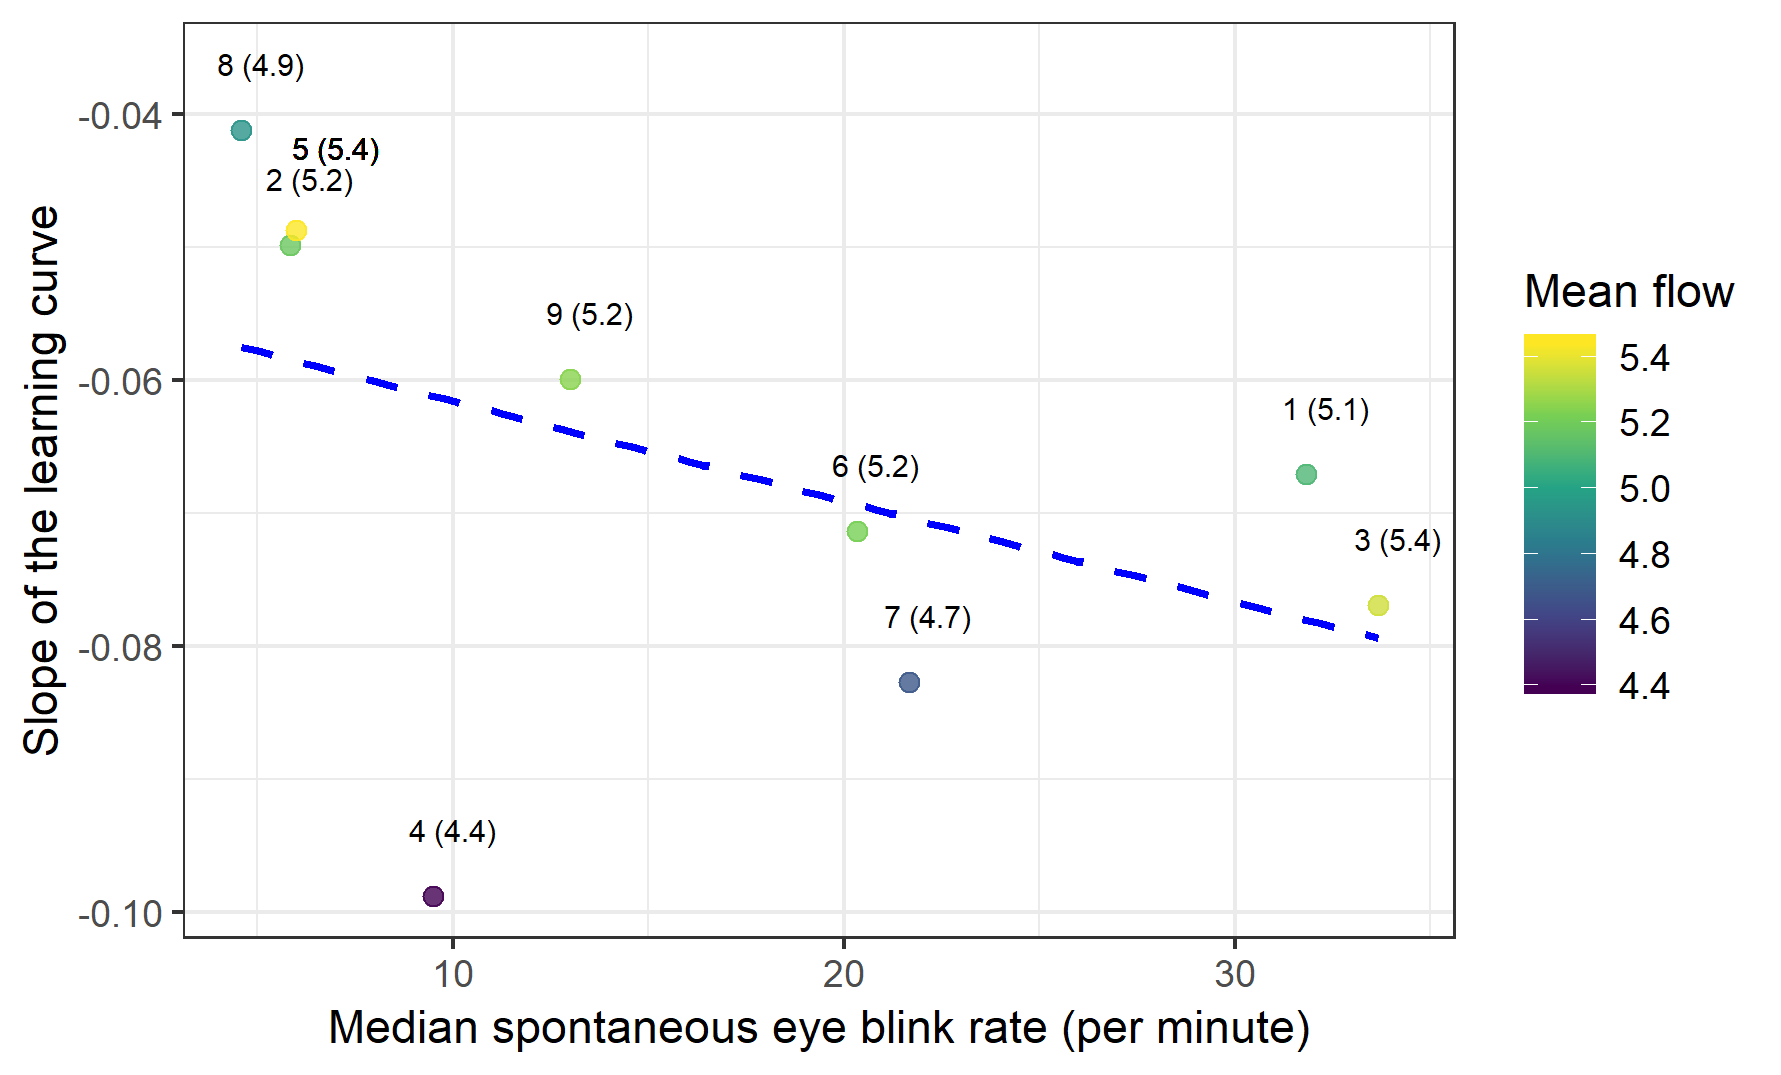
\includegraphics[width=\columnwidth]{lcurve_sbr_flowRL2}
	\caption{Participants' median spontaneous eye blink rate plotted against the slope of their learning curve, and coloured by their mean Flow scores. Linear model is depicted by the dashed line. Each point is labelled with the participant number (1..9) and exact mean Flow score (in parentheses).}
	\label{fig:EBRvLC}
\end{figure}


% -0.859833

\begin{table}[!hb]
\centering
\caption{Outcome of simple-slopes analysis for Flow$\times$LC interaction: each row reports on the slope of LC slope at the level and value of Flow shown.}
\begin{tabular}{llllll}
\hline
Flow level & Flow & Est. & S.E. & t value & p \\
\hline
+ 1 SD & 5.40 & -1096.31 & 221.36 & -4.95 & 0.0002 \\
Mean   & 5.06 &  -683.33 & 143.15 & -4.77 & 0.0002 \\
- 1 SD & 4.73 &  -270.35 & 158.23 & -1.71 & 1.0 \\
\hline
\label{tab:simpslopes}
\end{tabular}
\end{table}

% SIMPLE SLOPES ANALYSIS
% Slope of LC when FM = 5.40 (+ 1 SD):
%      Est.   S.E. t val.    p
%  -1096.31 221.36  -4.95 0.00
% Slope of LC when FM = 5.06 (Mean):
%     Est.   S.E. t val.    p
%  -683.33 143.15  -4.77 0.00
% Slope of LC when FM = 4.73 (- 1 SD):
%     Est.   S.E. t val.    p
%  -270.35 158.23  -1.71 0.15
%
%  JOHNSON-NEYMAN INTERVAL

\subsection*{RQ2: blink rate and Flow components}
{\it session-wise within-subjects}



%%%%%%%%%%%%%%%%%%%%%%%%%%%%%%%%%%%%%%%%%%%%%%%%%%%%%%%%%%%%%%%%%%%%%%%%%%%%%%%%
%%%%%%%%%%%%%%%%%%%%%%%%%%%%%%%%%%%%%%%%%%%%%%%%%%%%%%%%%%%%%%%%%%%%%%%%%%%%%%%%
%%%%%%%%%%%%%%%%%%%%%%%%     DISCUSSION    %%%%%%%%%%%%%%%%%%%%%%%%%%%%%%%%%%%%%
\section{Discussion}
% exploration of Flow and on-task learning (LC as opposed to pre- post)
We present a longitudinal experiment of Flow in a game-like high-speed steering task where task performance is easily parametrised and its relation to Flow and sEBR analysed. % game was fairly successful in eliciting Flow-like experiences (high baseline, score five out of seven)
To induce Flow, the game was designed to hold the balance between skill and challenge constant: the difficulty of the game continually adapted to the skill level of the participant.

...

% Without aiming to propose a new model here, we can, based on our behavioural data, consider Flow and learning
{\it A possibly useful novel way to view Flow and learning is via task complexity. Flow has been proposed to be possible in {\it any} task, complex (e.g. car driving) or simple (e.g. dish washing) \cite{Csikszentmihalyi1999}, but has also been proposed to depend on perceived task value as well as challenge--skill balance \cite{Keller2012}. One way to resolve these ideas is to consider that the individual can {\it introduce} complexity (or value) to their activity if they appear to have exhausted a task's potential to challenge them. \cite{Nakamura2002} suggest such an exploratory mechanism to explain how individuals maintain Flow in complex tasks: ``As people master challenges in an activity...to continue experiencing flow, they must identify and engage progressively more complex challenges.'' The corollary for simple tasks is that individuals {\it create} complexity, e.g. with self-defined goals \cite{Rauterberg1995}. For example, a similar state to Flow, called the Zone, has been reported for machine-gambling addicts whose pastime is in fact skill-free, but who nevertheless believe that they are skilled \cite{Schull2014}.}

{\it In other words, complex tasks have deep structure to be learned, requiring non-trivial skill acquisition for any duration of learning and thus a shallow LC (learning is slow). Importantly, the skill level does not quickly peak, such as with simpler tasks like washing the dishes, where Flow might be obtained but cannot strongly interact with learning (without self-created complexity). Learning comes into play when we consider that the same task can appear at first simple and later complex, e.g. as our experiment game.}

% Relation to previous Work on eye blink rate
\subsection*{Learning, Flow, and sEBR}
Between-subjects evidence for RQ1 suggests a clear linear trend relating sEBR and LCs (Fig.~\ref{fig:EBRvLC}): the larger the sEBR, the steeper the LC slope (or: the higher the LC intercept). The distance of data-points from the fitted model values also closely match the distribution of Flow mean scores, meaning that individuals with lowest Flow also diverge the most from the sEBR$\times$LC model. Interaction analysis then supports the idea that sEBR correlation with LC is stronger the higher the mean Flow. We thus claim that there is a genuine sEBR--LC relationship that is moderated by Flow. We cannot decide causality based on our data, but there is literature relevant to mechanisms, that can help identify future directions of inquiry.

Learning is influenced both by psychological factors (motivation, prior experience) and physio-/neurological factors. One potentially relevant factor for studying Flow and skill acquisition is the well-established relationship between attention and striatal dopamine levels \cite{Dreisbach2005}. The striatum plays a major role in decision making and reward/aversion processing, moderated by the level of tonic dopamine D2-receptors therein; the postsynaptic levels of dopamine can thus bias the entire learning process. This is illustrated for example in studies of `attentional blink' (AB) by Slagter and others \cite{Slagter2012,COLZATO2008}), which suggest a U-shaped function between tonic striatal dopamine and AB size. In other words, very high or low levels of dopamine D2-receptor density can make attention updating too rapid (distractable) or too slow (inattentive).

sEBR has been suggested as an externally-measurable index of striatal dopamine level (though caution is needed, see \cite{dang2017spontaneous}). Early work by \cite{Karson1983} linked sEBR to striatal dopamine in humans and other primates. \cite{Taylor1999} then localised to the caudate nucleus, whose normal function is implicated in classification learning \cite{Seger2005}; caudate nucleus volumetric asymmetry is implicated in inattention symptomatology \cite{Schrimsher2002}. Later work from \cite{Slagter2015} has shown that sEBRs may relate specifically to avoidance learning; others have linked dopamine levels and sEBR to perseverance, distractibility and cognitive control \cite{Muller2007,Dreisbach2005}. Finally, \cite{DeManzano2013} have shown that  predisposition to experience Flow is positively correlated with striatal dopamine D2-receptor availability (measured in PET), specifically in caudate and putamen, and stronger in right hemisphere than left.

Let us consider learning as a process whereby perception, cognition and action become attuned to task demands. In our game task, learning involves high-frequency decision making with respect to continuously updating stimuli of uniform kind (not unlike AB task, a continuous performance test designed to probe AB size \cite{Slagter2012}). In this view, the sEBR--LC relationship could be interpreted as showing that higher D2 density indexed by sEBR supports learning (LC slope). An alternative interpretation is that it reflects higher distractability in the early phases of learning (LC intercept).

The underlying mechanism could be that higher dopamine levels permit more rapid attention updating and thus more fluid response to changing task demands. This can work despite \cite{Slagter2012}'s proposed U-shaped function: because our game-task constantly maintains a level of demand slightly greater than the participants' skill. Thus, in this context, higher sEBR tends to be better, possibly because the {\it requirement} for rapid attention updating grows with the learned task skill.

Less subjective Flow was reported by those participants who deviated (positively or negatively) from this relationship. Lower Flow could be due to, e.g., misalignment of task demands and attentional updating rate, creating a more effortful experience. So the observed moderation by Flow scores of the sEBR--LC relationship could be speculated to have a basis in adjusting attention updating, in response to changing task speeds, physiologically underpinned by the nigro-striatal DA system. In other words, it may not be the case that an absolute level of striatal dopamine should predict learning, but rather an individual level relative to how each participant relates to the task (vis-\'{a}-vis gaming experience, motivation, fine motor skills, or potentially many other variables). If a participant's tonic dopamine is not at their ideal level for this task, they might nevertheless do well in the task, and yet find the experience more effortful and less fluid (than is suggested as Flow-like by wording of the FSS).


\subsection{Limitations and Future Work}
{\it Our study had a small convenience sample because (a) the recording paradigm was extensive (around eight hours of contact time), and (b) it was to some degree an exploratory study; both implying the need to constrain datasets to tractable sizes. It is worth noting that while we recruited only 9 participants, we collected a significant amount of behavioural and physiological data for each participant over a course of two weeks and 8 recording sessions. This amounts to a particularly rich dataset allowing us to dig deep into the underpinnings of skilled high speed steering and Flow. Moreover, given the fact our experimental paradigm has not been used previously, we could not {\it a priori} easily estimate the statistical power required to discover significant effects. However, our results ended up being both strikingly {\it similar} and {\it strong} within each participant, suggesting that collecting a larger sample size would likely have {\it not} changed the pattern of the results or provided more in-depth insights. Regardless of the justifications, the sample size and method are minor limitations to be remedied in future work. Additionally, lacking experimental manipulations the study cannot make strong causal claims, which could be improved by recording separate conditions of the game task, e.g. with varied difficulty levels.}

{\it Trial-by-trial analysis is limited by the Flow self-report which only has one data point per trial. It would be more powerful to analyse {\it inside} each trial. In our data, self-reported Flow is a point model of an entire trial, for which the participant knows their score. Self-reported Flow is thus an after-the-fact report, and could be criticized for not capturing the in-the-moment {\it experience of Flow}, which might fluctuate greatly during a trial. Analysing the fluctuation of Flow-experience requires us to model individual actions and/or their outcomes, and sample Flow during performance. This is a difficult challenge, because paying attention to one's phenomenal state might easily disrupt the very processes sustaining that state, especially for Flow which is unreflective by definition. Future work should aim to model the conditions of Flow ({\sf C1--3}) in real-time, while simultaneously recording participant physiology, to uncover in greater detail the relationships involved. The existing dataset will be used for this purpose, in a pending report on the biosignals recorded with high temporal resolution, primarily electro-dermal activity.}

To further explore the possible role of striatal dopamine, it would be interesting to experimentally manipulate the game to adjust the distance between obstacles, thus altering the attention-updating rate required to navigate without collisions (motor precision variation can be minimised by a suitably long training period). This manipulation could be varied in response to measurements of sEBR (which can be automated, e.g. by using electro-oculography \cite{toivanen2014}), to systematically investigate whether sEBR holds explanatory power with respect to individual variability in learning.


\subsection{Conclusion}

% We report evidence that the LC across sessions is predicted by participants' spontaneous blink rate.
We report evidence that slope of the learning curve (total play time about 2 h, distributed over two weeks) is predicted by the participants' spontaneous blink rate, moderated by global Flow. This relationship potentially indicates a role for striatal dopamine in learning the visuomotor steering task, which may interact with the experience of Flow.

Understanding how perceptual-cognitive and motor processes underlying performance give rise to phenomenological experiences, such as Flow, and how the phenomenal experiences relate to performance on the other is an important topic for understanding human motivation and performance. This study contributes to this goal and we hope will inspire more inquiry into the dynamics of the Flow experience in different stages of learning a skill.


%%%%%%%%%%%%%%%%%%%%%%%%%%%%%%%%%%%%%%%%%%%%%%%%%%%%%%%%%%%%%%%%%%%%%%%%%%%%%%%
%%%%%%%%%%%%%%%%%%%%%%%%%%%%%%%%%%%%%%%%%%%%%%%%%%%%%%%%%%%%%%%%%%%%%%%%%%%%%%%%
%%%%%%%%%%%%%%%%%%%%% POST-HOC MATERIAL OF VITAL IMPORTANCE %%%%%%%%%%%%%%%%%%%%


\section{Acknowledgements}
We thank Kalle Toika and Juha Veps\"{a}l\"{a}inen (JV below).

\section*{Author contributions statement}
% please edit as appropriate
OL, JP and BUC conceived the study.
OL helped design the gameplay.
BUC and TT designed and implemented the data collection.
NL, TT, PP, RF, VPI, and JP translated the FSS.
All authors participated in decisions on the experiment specifications.
RF, VPI, NL, PP, and TT conducted the experiment.
BUC, VPI, TT, RF, PP, NL, JP, and OL analysed and interpreted the results.
BUC, JP and OL drafted the paper.
All authors participated in writing and reviewing, and approved the manuscript.


\bibliographystyle{apacite}

\setlength{\bibleftmargin}{.125in}
\setlength{\bibindent}{-\bibleftmargin}

\bibliography{CogCarFlow_bib}

\end{document}
